%!TEX root = ../PhDthesis.tex
\chapter{Exploring the role of inhibition in surround modulation}


\section{Methods}

\subsection{The LESPI model}

\textbf{L}ong-\textbf{R}ange \textbf{E}xcitation, \textbf{S}sst and
\textbf{PV} \textbf{I}nhibition (LESPI) model again builds on the
previous models introducing an additional population of inhibitory
neurons, which is entirely recurrently driven via short- and
long-range projections by the two other populations. The diagram in
\ref{LESPIDiagram} shows how the three populations of V1 neurons are
recurrently connected.

The influence of the aggregate long-range excitatory and di-synaptic
inhibition via the Sst population is expressed as an additional
multiplicative factor modulating the response of the excitatory
neurons. The response of the excitatory population is then given by:

\begin{equation}
  \eta_{exc} = \frac{\eta_{A} + \eta_{LOC}}{1 + \eta_{PV}} * \eta_{SM}
\end{equation}

where $\eta_{A}$ is the LGN afferent activity, $\eta_{LOC}$ the local
excitatory contribution, $\eta_{P}$ the PV inhibitory contribution
and the surround modulation term $\eta_{SM}$ is defined as:

\begin{equation}
  \eta_{SM} = 1 + \eta_{LAT} - \eta_{S}
\end{equation}

where $\eta_{LAT}$ represents the long-range lateral excitatory
contribution and $\eta_{S}$ is the Sst inhibitory contribution. In the
SEPI model the $\eta_{SM}$ term simply reduces to 1, eliminating all
long-range interactions. The surround modulatorion term provides gain
when excitation exceeds inhibition and shunting inhibition when the
reverse is true. As such, this term provides a convenient abstraction
to model the modulatory influence of the dendritic integration of
long-range inputs.

The effective excitatory gain may not be a bad approximation to the
effect of long-range horizontal connections, which have been shown to
be strongly voltage dependent \citep{Hirsch1991}. Since Sst neurons
generally target distal dendrites they have generally been associated
with subtractive inhibition, they do however also have a
multiplicative component \citep{Wilson2012}. Additionally, their
preference for targetting distal dendrites may allow them to
effectively gate horizontal excitatory and feedback inputs
\citep{Ma2011, Gentet2012}. Additionally theoretical studies indicate
active dendritic spike backpropagation can lead to multiplicative
increases in gain, while reduction in spike backpropagation can lead
to divisive scaling of the firing rate \citep{Mehaffey2005}.

\begin{figure}
	\centering
        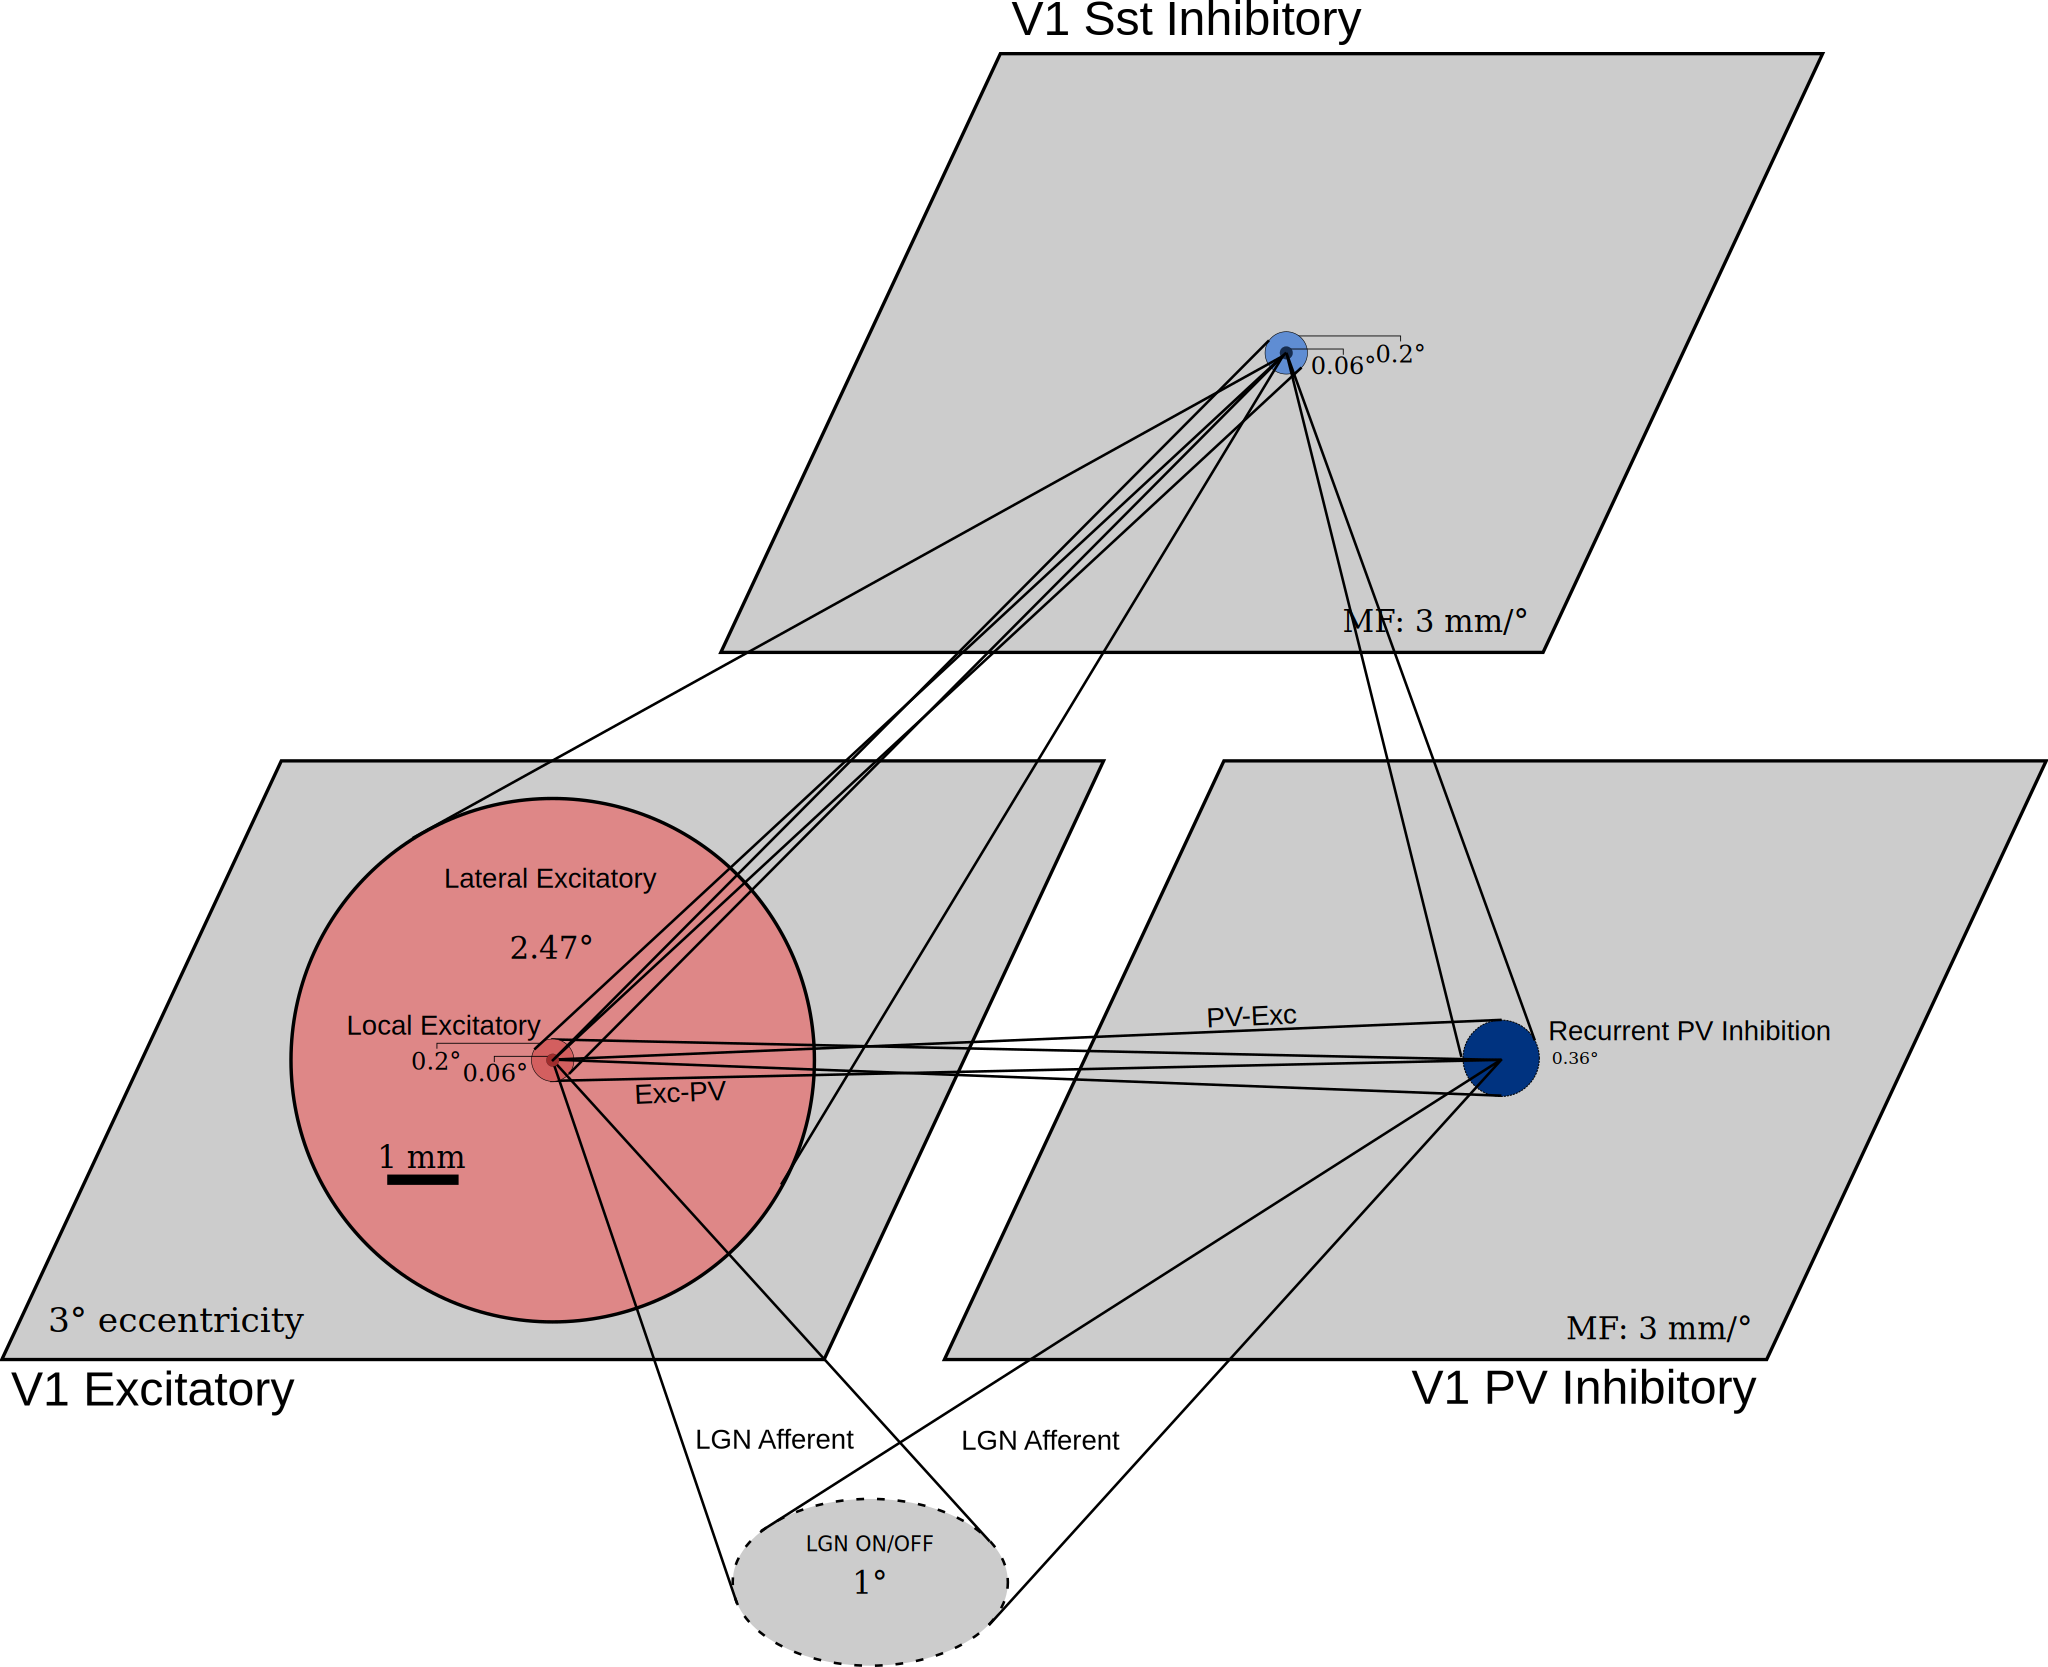
\includegraphics[width=1.0\textwidth]{LESPI_Diagram.pdf}
	\caption{Diagram of the LESPI V1 stage of the model showing the
          spatial scales of the various excitatory (red) and
          inhibitory (blue) connections. Satured colors indicate the
          kernel radii, while lightly shaded regions indicate kernel
          cut-off extents.}
	\label{LESPIDiagram}
\end{figure}



\begin{figure}
	\centering
	\includegraphics[width=1.0\textwidth]{./v1circuit.pdf}
	\caption[]{High-level circuit diagram of the LESPI model.}
    \label{circuit_diagram}
\end{figure}


\subsection{Surround modulation}

Beyond measuring simple attributes of the spatial organization in LGN
and V1, higher order effecs can be explored through complex surround
modulation measurement protocols. In addition to the simple area
summation curve measurements described above we replicate two further
protocols to evaluate the spatial response properties of the model.
In particular we are interested in the interaction between the spatial
arrangement of visual patterns presented to an animal and the contrast
on the response properties of visually responding neurons. For that
purpose we replicate two measurement protocols, a simple annulus based
contrast suppression measurement \cite{Jones2002} and a protocol using
target and flanker stimuli performed by \cite{Kapadia1995}.

\paragraph{Orientation contrast suppression}

The orientation contrast suppression is perhaps one of the most well
studied surround modulation paradigms. The measurement involves
presenting stimuli of a central sine grating, optimized to the
preferred size, frequency and orientation of the neuron being
measured. Once the baseline activity has been measured an additional
surround anulus with the same frequency is added and varied in
contrast, size and orientation to measure orientation dependent
interactions between center and surround (as shown in Figure
\ref{ORC_Stimulus}).

\begin{figure}
	\centering
        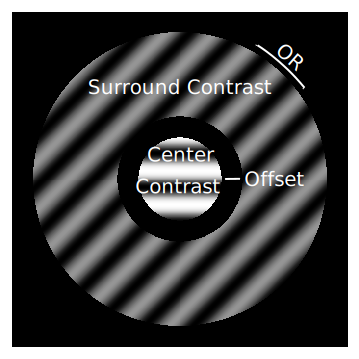
\includegraphics[width=0.5\textwidth]{ORC_Stimulus.pdf}
	\caption{Orientation contrast stimulus measuring modulation by a
      sine grating annulus on the response of a central neuron
      responding to a central sine grating disk of the same frequency.
      Stimulus is varied by center and surround contrast, surround
      orientation and the offset between the central disk and the
      surround annulus.}
	\label{ORC_Stimulus}
\end{figure}

The surround facilitation is quantified as:

\begin{equation}
F = (\frac{R_{cs}}{R_c} - 1) * 100
\end{equation}

where $R_{CS}$ is the response of the combined stimulus and $R_C$ the
response to just the center stimulus.

\paragraph{Flanker Modulation}

Instead of working solely using area based protocols we also make use
of a simple bar based stimulus along with a flanker, which is
modulated in a number of ways to characterize the surround modulation
effects associated with this protocol. In \cite{Kapadia1995} describe
a high degree of variability ranging from a complete lack of surround
modulation to facilitation and suppression. The three stimulus
protocols employed here are shown in \ref{Flanker}, we replicate these
protocol on the model to compare the effects observed in experiments
qualitatively.

\begin{figure}
	\centering
        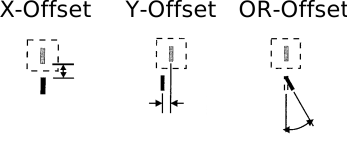
\includegraphics[width=1.0\textwidth]{FlankerProtocol.pdf}
	\caption{Flanker offset surround modulation paradigm. Measuring
      the effect of a flanker stimulus varying by an offset in X, Y
      and orientation on the response of a neuron to a target
      stimulus.}
	\label{Flanker}
\end{figure}
